\documentclass[12pt]{article}
\usepackage[utf8]{inputenc}
\usepackage[french]{babel}
\usepackage[T1]{fontenc}
\usepackage{amsmath}
\usepackage{amsfonts}
\usepackage{amssymb}
\usepackage{graphicx}
\usepackage{relsize}
\usepackage{subcaption}
\usepackage{amsmath}
\usepackage{listings}
\usepackage{listingsutf8}
\usepackage{xcolor}
\usepackage{multicol}
\usepackage{blindtext}
\usepackage{geometry}
 \geometry{
 a4paper,
 total={170mm,257mm},
 left=20mm,
 top=20mm,
 }
\hyphenpenalty=5000
\graphicspath{{../Beamer/Affiche/0-ReconnaissanceVocale/}{../Beamer/Affiche/1-Introduction/}{../Beamer/Affiche/2-Activation-Gradient/}{../Beamer/Affiche/4-XOR/}{../Beamer/Affiche/5-MNIST/}{../Beamer/Affiche/6-Mot/}{../Beamer/Affiche/7-Vocal/}}


\author{TRAN-THUONG Tien-Thinh}
\title{Reconnaissance vocale lors d’appel d’urgence grâce à un réseau de neurones}
\date{2021-2022}

\begin{document}
\maketitle
\begin{abstract}
    D'après le ministère de la Santé : \\
    Il y a eu plus de \textbf{31 millions} d'appels d'urgence en 2018. Seuls \textbf{69\%} des appels étaient décrochés dans la minute. \break
    \indent Objectif :\\
    Utiliser la reconnaissance vocale par réseau de neurones pour aider à classifier rapidement l'objet d'un appel.
\end{abstract}
\rule{\linewidth}{.5pt}

% 1-INTRODUCTION

\section{I - Introduction}
\begin{frame}{I - Introduction}
	\begin{block}{Présentation du modèle du perceptron}
		C'est  en 1943, que McCulloch et Pitts introduisent le modèle du perceptron.  \\
		Ce modèle est basé sur le fonctionnement du neurone humain.
	\end{block}
	\begin{figure}
		\centering
		\includegraphics[width=\textwidth]{2-Neurone.png}
		\caption{Schéma d'un neurone humain}
	\end{figure}
\end{frame}


\begin{frame}{I - Le perceptron}
	\begin{figure}
		\centering
		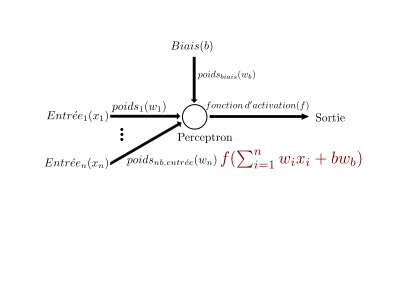
\includegraphics[width=\textwidth]{1-Perceptron.png}
		\caption{Schéma d'un perceptron}
	\end{figure}
\end{frame}


\begin{frame}{I - Représentation informatique}
	\begin{columns}
		\begin{column}[]{0.4\textwidth}
			\begin{center}
				$
					f
					\left(
					\begin{pmatrix}
						x_1 & \ldots & x_n & b
					\end{pmatrix}
					\times
					\begin{pmatrix}
						w_1    \\
						\vdots \\
						w_n    \\
						w_b
					\end{pmatrix}
					\right)
				$ \\
				\openup 1em
				La complexité est en $O(n)$
			\end{center}
		\end{column}
		\begin{column}[]{0.5\textwidth}
			\lstinputlisting[language=Python, firstline=15]{0-representation.py}
		\end{column}
	\end{columns}
	\caption{Représentation informatique du perceptron}
\end{frame}
% 2-Fonction d'activation
\section{II - Fonction d'activation}
\begin{frame}{II - Fonction d'activation}
	\begin{block}{Fonction d'activation}
		Sans fonction d'activation, le neurone sans fonction d'activation est multilinéaire par rapport à ses entrées. \\
		\openup 1em
		Les fonctions d'activation permettent une classification non linéaire.
	\end{block}
	\openup 2em
	\begin{figure}
		\centering
		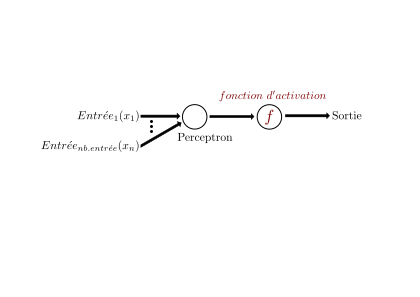
\includegraphics[width=\textwidth]{8-activation.png}
		\caption{Utilisation de la fonction d'activation}
	\end{figure}
\end{frame}


\begin{frame}{II - Fonction d'activation}
	\begin{figure}
		\begin{subfigure}[]{0.3\textwidth}
			\includegraphics[width=90px]{0-Sigmoide.png}
			\caption{Sigmoïde}
		\end{subfigure}
		\begin{subfigure}[]{0.3\textwidth}
			\includegraphics[width=90px]{0-Tanh.png}
			\caption{Tanh}
		\end{subfigure}
		\begin{subfigure}[]{0.3\textwidth}
			\includegraphics[width=90px]{0-ReLU.png}
			\caption{ReLU}
		\end{subfigure}
	\end{figure}
	\begin{block}{}
		\centering
		\begin{tabular}{ l || c | c | }
			Fonction                            & Formule                                          & Dérivée                                    \\ \hline \\
			Sigmoïde (a)                        & $\mathlarger{\frac{1}{1+e^{-x}}}$                & $f(x) \times (1-f(x))$                     \\ \\
			Tangente Hyperbolique (Tanh) (b)    & $\mathlarger{\frac{e^{x}-e^{-x}}{e^{x}+e^{-x}}}$ & $1-f(x)^2$                                 \\ \\
			Unité Linéaire Rectifiée (ReLU) (c) & $max(0, x)$                                      & $ \left\{\begin{array}{ll}
					0 & \mbox{si } x<0 \\
					1 & \mbox{sinon }\end{array}\right.$ \\
		\end{tabular}
	\end{block}
\end{frame}


\begin{frame}{II - Fonction d'activation : Sigmoïde}
	\begin{figure}
		\centering
		\includegraphics[width=250px]{0-Sigmoide.png}
		\caption{Sigmoïde}
	\end{figure}
\end{frame}


\begin{frame}{II - Fonction d'activation : TANH}
	\begin{figure}
		\centering
		\includegraphics[width=250px]{0-Tanh.png}
		\caption{TANH}
	\end{figure}
\end{frame}


\begin{frame}{II - Fonction d'activation : ReLu}
	\begin{figure}
		\centering
		\includegraphics[width=250px]{0-ReLU.png}
		\caption{ReLu}
	\end{figure}
\end{frame}
% 3-Descente de gradient

\section{III - Descente de gradient}
\begin{frame}{III - Descente de gradient}
    \begin{block}{Descente de gradient}
        La Descente de Gradient est un algorithme d’optimisation qui permet de trouver un minimum local d'une fonction en convergeant progressivement. \\
        Dans l'apprentissage des réseaux de neurones, la descente de gradient est utilisée pour trouver le minimum d'une fonction "coût", évaluant l'erreur entre la valeur de sortie du réseau et celle attendue. \\
        Cette fonction d'erreur est noté $f : s \mapsto (s - s_{attendue})^2$, avec $s$ la sortie donnée par le modèle et $s_{attendue}$ la sortie cible. \\
        En effet, trouver des paramètres (poids, architecture du réseau, fonction d'activation) permettant d'avoir une erreur nulle revient à résoudre le problème qu'évalue cette fonction coût par rapport aux données d'entrée.
    \end{block}
\end{frame}

\begin{frame}{III - Descente de gradient}
    \begin{block}{Algorithme du gradient}
        Soit $n \in \mathbb{N}, \varepsilon > 0$. On munit $\mathbb{R}^n$ de son produit scalaire canonique. \\
        Soit $f$ une fonction différentiable de $\mathbb{R}^n \to \mathbb{R}$. \\
        Soit $x_0$ une valeur initiale aléatoire, $t$ le taux d'apprentissage. \\
        Supposons $x_0, \ldots, x_k$ construits. \\
        • Si $\norme{\nabla f(x_k)} \leq \varepsilon$, on s'arrête. \\
        • Sinon on pose $x_{k+1} = x_k - t \nabla f(x_k)$ \\
    \end{block}
    
    \begin{figure}
        \centering
        \includegraphics[height=75px]{1-DescenteGradient.jpg}
        \caption{Descente de Gradient pour $f(x) = (x-0.75)^2$; $x_0=0.1$ et $\varepsilon = 0.1$}
    \end{figure}
\end{frame}

\begin{frame}{III - Importance du choix du taux d'apprentissage}
    Pour la suite on continuera avec la fonction $f(x) = (x-0.75)^2$ et $x_0=0.1$. \\
    On montre qu'en choisissant un taux d'apprentissage trop petit ou trop grand, il est possible que la descente de gradient diverge, ou ne converge pas assez vite.
    \begin{figure}
        \centering
        \includegraphics[height=80px]{2-DescenteGradient.jpg}
        \caption{Descente de Gradient on force l'arrêt à $k=8$}
    \end{figure}
\end{frame}

\begin{frame}{III - Utilisation du Moment}
    \begin{block}{III - Descente de gradient avec moment}
        $x_0$ aléatoire et le moment $\omega_0 = 0$.
        Supposons $x_0, \ldots, x_k$ et $\omega_0, \ldots, \omega_k$ construits. \\
        • On pose $\omega_{k+1} = \gamma \omega_k + t \nabla f(x_k)$ \\
        • On pose $x_{k+1} = x_k - \omega_{k+1}$
    \end{block}
    \begin{figure}
        \centering
        \includegraphics[height=130px, trim=0 35 0 35, clip]{3-Moment.jpg}
        \caption{Descente de gradient SANS/AVEC moment où $\gamma = 0.5$, arrêt à $k=4$}
    \end{figure}
\end{frame}

\begin{frame}{III - Utilisation du Moment}
    Voici, une simulation pour des taux d'apprentissage "trop grand" ou "trop petit".
    \begin{figure}
        \centering
        \includegraphics[height=130px, trim=0 35 0 35, clip]{4-Moment.jpg}
        \caption{Descente de gradient SANS/AVEC moment où $\gamma = 0.5$, arrêt à $k=8$}
    \end{figure}
\end{frame}

\begin{frame}{III - Utilisation du Moment}
    Le moment permet également de s'échapper de certains minima locaux.
    \begin{figure}
        \centering
        \includegraphics[width=\textwidth, trim=0 10 0 10, clip]{5-Moment.jpg}
        \caption{Descente de gradient SANS/AVEC moment où $\gamma = 0.5$, arrêt à $k=8$}
    \end{figure}
\end{frame}

\begin{frame}{III - Apprentissage stochastique ou par paquet (Batch)}
    Les paramètres du réseau de neurones sont les poids qui pondèrent l'entrée. C'est sur eux que l'on opèrent la descente de gradient. 
    \begin{figure}
        \centering
        \includegraphics[width=\textwidth]{1-DescenteGradient.jpg}
    \end{figure}
    \begin{figure}
        \centering
        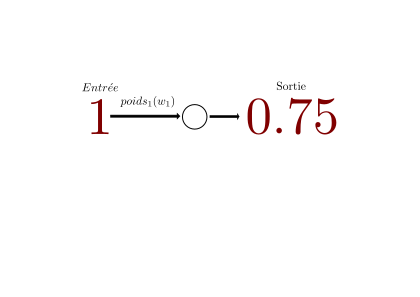
\includegraphics[height=50px]{6-Perceptron.png}
        \caption{Schéma du perceptron linéaire}
    \end{figure}
\end{frame}

\begin{frame}{III - Apprentissage stochastique ou par paquet (Batch)}
    \begin{multicols}{2}
        Il faut prendre en compte le fait que les données d'apprentissage ne sont pas toujours exactes, elles sont forcément inscrites dans une marge d'erreur. 
        \columnbreak
        $
            \left< f
            \left(
            \begin{pmatrix}
                    x_1^{1} & \ldots & x_n^{1} & b      \\
                    \vdots  & \vdots & \vdots  & \vdots \\
                    x_1^{D} & \ldots & x_n^{D} & b
                \end{pmatrix}
            \times
            \begin{pmatrix}
                    w_1    \\
                    \vdots \\
                    w_n    \\
                    w_b
                \end{pmatrix}
            \right) \right>
        $
    \end{multicols}
    \begin{figure}
        \centering
        \includegraphics[width=\textwidth, trim=0 30 0 30, clip]{7-Batch.jpg}
        \caption{Comparaison apprentissage stochastique et par paquet, $f(x) = (x-0.75)^2$}
    \end{figure}
\end{frame}

% 4-Problème de reproduction de l'opérateur XOR

\section{IV - Problème de reproduction de l'opérateur XOR}
\begin{frame}{IV - Problème de reproduction de l'opérateur XOR}
	\begin{block}{Problème non linéairement séparables}
		Une couche de perceptron ne peut pas reproduire les opérateurs non linéairement séparables. \\
		Il faut mettre des couches de perceptron en série (couches cachées) pour pouvoir reproduire ces opérateurs. \\
	\end{block}
	\begin{figure}
		\centering
		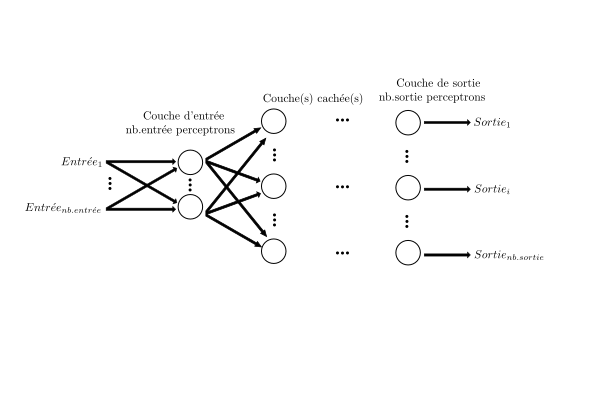
\includegraphics[height=120px]{1-Reseau.png}
		\caption{Schéma d'un réseau de neurones}
	\end{figure}
\end{frame}


\begin{frame}{IV - Problème de reproduction de l'opérateur XOR}
	\begin{block}{Le XOR nécessite un réseau}
		Le XOR, \og $ou\ exclusif$ \fg, est un opérateur non linéairement séparable. \\
	\end{block}
	\begin{figure}
		\centering
		\includegraphics[width=150px]{2-XOR.jpg}
		\caption{Schéma de l'opérateur XOR}
	\end{figure}
\end{frame}


\begin{frame}{IV - Problème de reproduction de l'opérateur XOR}
	\begin{figure}
		\centering
		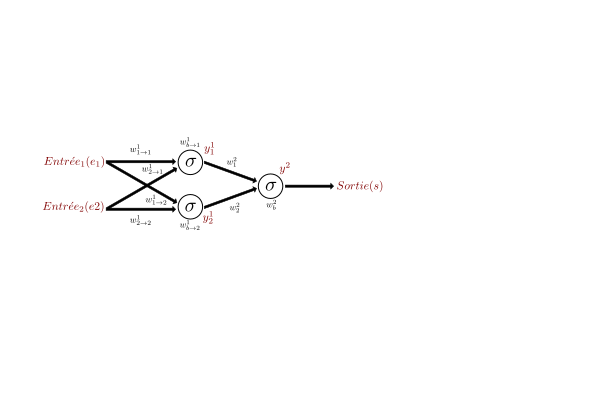
\includegraphics[width=230px]{3-Model.png}
		\caption{Schéma du réseau de neurone reproduisant le XOR}
	\end{figure}
	\begin{block}{Descente de gradient}
		$w \leftarrow w - t \dfrac{\partial f}{\partial w}$ où $t$ est le taux d'apprentissage et $f$ la fonction de coût
	\end{block}
	\begin{exampleblock}{Exemple}
		• $\dfrac{\partial f}{\partial w^2_1} = 2(s - s_{attendue})\sigma_2 'y^1_1$ \\
		• $\dfrac{\partial f}{\partial w^1_{1\to 1}} = 2(s - s_{attendue})\sigma_2 'w^2_1 \sigma _{1} ' e_{1}$
	\end{exampleblock}
\end{frame}


\begin{frame}{IV - Code}
	\lstinputlisting[language=Python, firstline=15]{1-XOR.py}
\end{frame}


\begin{frame}{IV - Apprentissage de la reproduction du XOR}
	\begin{figure}
		\centering
		\includegraphics[width=270px]{4-XOR.png}
		\caption{Erreur sur la reproduction du XOR au cours de l'apprentissage}
	\end{figure}
\end{frame}


\begin{frame}{IV - Mes résultat}
	\begin{block}{Données}
		• 4 données \\
		• 300 générations \\
		• Erreur minimale atteinte 0.036
	\end{block}
	\begin{align*}
		Entr\acute{e} e\, :
		\begin{pmatrix}
			0 & 0 \\
			0 & 1 \\
			1 & 0 \\
			1 & 1
		\end{pmatrix}
		 & \to
		\mathlarger{\mathlarger{\sigma_{couche1}}}
		\left( \centerdot \times
		\begin{pmatrix}
				0.85 & 5.42 \\
				0.85 & 5.40 \\
				0.14 & 0.44
			\end{pmatrix}
		\right) \\
		 & \to
		\mathlarger{\mathlarger{\sigma_{couche2}}}
		\left( \centerdot \times
		\begin{pmatrix}
				-18.39 \\
				14.42  \\
				0.02
			\end{pmatrix}
		\right) \\
		 & \to
		Sortie\, :
		\begin{pmatrix}
			0.12 \\
			0.81 \\
			0.81 \\
			0.24
		\end{pmatrix}
		Sortie_{attendue}\, :
		\begin{pmatrix}
			0 \\
			1 \\
			1 \\
			0
		\end{pmatrix}
	\end{align*}
\end{frame}
% 5-MNIST

\section{V - MNIST}
\begin{frame}{V - Reconnaissance d'image}
	\begin{block}{Problématique : Reconnaissance des chiffres écrits à la main}
		Images de taille $28 \times 28$ pixels en noir et blanc : \\
		\quad - 60 000 images pour l'entrainement. \\
		\quad - 10 000 autres pour la vérification.
	\end{block}
	\begin{figure}
		\centering
		\includegraphics[width=150px]{1-mnist.jpg}
		\caption{Exemple d'images}
	\end{figure}
\end{frame}


\begin{frame}{V - Apprentissage d'un problème de classification}
	On prend un réseau de neurones avec $28 \times 28 = 784$ entrées, et 10 sorties. \\
	\begin{block}{Softmax}
		La fonction d'activation softmax permet de normaliser en probabilités les sorties : \\
		• $p_i = \frac{exp(a_i)}{\sum_{k=1}^{n}exp(a_k)}$ la probabilité de la sortie $a_i$ \\
		• $\dfrac{\partial p_i}{\partial a_j} = p_i\times(\delta_{ij}-p_j)$ \\
	\end{block}
	\begin{block}{Cross-entropy}
		La fonction coût des problèmes de classification est Cross-entropy : \\
		• $L\ \ \ = -\sum_{k=1}^{n}y_ilog(p_i)$ avec $y_i$ la sortie attendue \\
		• $\dfrac{\partial L}{\partial a_i} = p_i - y_i$
	\end{block}
\end{frame}


\begin{frame}{V - Softmax}
	\begin{figure}
		\centering
		\includegraphics[height=150px]{2-Softmax.png}
		\caption{Schéma d'utilisation du Softmax}
	\end{figure}
\end{frame}


\begin{frame}{V - Mes résultats}
	\begin{columns}[T] % align columns
		\begin{column}{.52\textwidth}
			\begin{figure}
				\centering
				\includegraphics[width=\textwidth]{3-Apprentissage.jpg}
				\caption{Courbes d'apprentissage}
			\end{figure}
		\end{column}
		\hfill
		\begin{column}{.50\textwidth}
			\bigskip	\bigskip	\bigskip
			\bigskip	\bigskip	\bigskip
			\bigskip	\bigskip	\bigskip
			Taux de bonnes réponses après 100 générations d'entrainement : \\
			- 91.5\% sur les données d'entrainement \\
			- 91.3\% sur les données de validation. \\
		\end{column}%
	\end{columns}
\end{frame}


\begin{frame}{V - Mes résultats}
	\begin{figure}
		\centering
		\includegraphics[height=200px]{4-Resultat.jpg}
		\caption{Exemple sur un échantillon de 40 images de validation}
	\end{figure}
\end{frame}


\begin{frame}{V - Convolution d'image}
	\begin{figure}
		\centering
		\includegraphics[width=\textwidth]{5-convolution.png}
		\caption{Schéma de la convolution d'image $O(0, 0) = \sum_{i=0}^{2}\sum_{j=0}^{2}I(i, j)\times F(i, j)$}
	\end{figure}
\end{frame}


\begin{frame}{V - Convolution d'image}
	\begin{columns}[T] % align columns
		\begin{column}{.4\textwidth}
			\includegraphics[width=\textwidth]{6-cat.jpg}
			\includegraphics[width=\textwidth]{6-dog.jpg}
			\begin{exampleblock}{Détection de contour}
				\begin{center}
					\centering
					$
					F =
					\begin{pmatrix}
						-1 & -1 & -1 \\
						-1 & 8  & -1 \\
						-1 & -1 & -1
					\end{pmatrix}
					$
				\end{center}
			\end{exampleblock}
		\end{column}
		\hfill
		\begin{column}{.58\textwidth}
			\lstinputlisting[language=Python, firstline=15]{4-convolve.py}
		\end{column}
	\end{columns}
\end{frame}


\begin{frame}{V - Utilisation de réseau de neurones convolutif}
	\begin{columns}[T]
		\begin{column}{.70\textwidth}
			\begin{figure}
				\centering
				\includegraphics[width=\textwidth]{7-Resultat.jpg}
				\caption{Exemple sur un échantillon de 40 images $Fashion\ MNIST$}
			\end{figure}
		\end{column}
		\hfill
		\begin{column}{.30\textwidth}
			\bigskip	\bigskip	\bigskip
			\lstinputlisting[language=Python, firstline=15]{6-fashionDico.py}
		\end{column}
	\end{columns}
\end{frame}

% 6-Reconnaissance de mot

\section{VI - Reconnaissance de mot}
\begin{frame}{VI - Reconnaissance de mot}
Un moyen simple de reconnaitre un mot est d'en faire le spectrogramme puis de résoudre le problème de reconnaissance comme si cela était une image. \\
Le site du gouvernement recense ces mots clés pour les appels d'urgences : \\
\begin{enumerate}
  \item[15] malaise, hémorragie, brûlure, intoxication
  \item[17] violences, agression, vol, cambriolage
  \item[18] incendie, gaz, effondrement, électrocution
\end{enumerate}
\begin{figure}
	\begin{subfigure}[]{0.3\textwidth}
		\includegraphics[width=90px]{1-Incendie.jpg}
  		\caption{INCENDIE}
	\end{subfigure}
	\begin{subfigure}[]{0.3\textwidth}
		\includegraphics[width=90px]{1-Intoxication.jpg}
  		\caption{INTOXICATION}
	\end{subfigure}
	\begin{subfigure}[]{0.3\textwidth}
		\includegraphics[width=90px]{1-Cambriolage.jpg}
		\caption{CAMBRIOLAGE}
	\end{subfigure}
\end{figure}
\end{frame}

\section{VII - Reconnaissance vocale}
\begin{frame}{VII - Reconnaissance vocale}
Découpage en élément lexicaux, puis décodage du mot.
\begin{figure}
	\begin{subfigure}[]{0.3\textwidth}
		\includegraphics[width=90px]{1-A.jpg}
  		\caption{A}
	\end{subfigure}
	\begin{subfigure}[]{0.3\textwidth}
		\includegraphics[width=90px]{1-E.jpg}
  		\caption{E}
	\end{subfigure}
	\begin{subfigure}[]{0.3\textwidth}
		\includegraphics[width=90px]{1-I.jpg}
		\caption{I}
	\end{subfigure}
\end{figure}
\begin{figure}
	\begin{subfigure}[]{0.3\textwidth}
		\includegraphics[width=90px]{1-O.jpg}
  		\caption{O}
	\end{subfigure}
	\begin{subfigure}[]{0.3\textwidth}
		\includegraphics[width=90px]{1-U.jpg}
  		\caption{U}
	\end{subfigure}
	\begin{subfigure}[]{0.3\textwidth}
		
\includegraphics[width=90px]{2-Matching.png}
	\end{subfigure}
\end{figure}
\end{frame}


\end{document}


